\documentclass[wmii,inf,inz]{uwmthesis} % Wybór klasy dokumentu
\usepackage[polish]{babel}
\usepackage{hyperref} % Dodanie obsługi hiperłączy
\usepackage[T1]{fontenc} % Obsługa polskich znaków w czcionkach
\renewcommand{\labelitemi}{\textbullet}  % Standardowa kropka
\usepackage{enumitem}
\usepackage{graphicx}
\newenvironment{indenteditemize}
{\begin{itemize}[left=1cm]} % zmień wartość '2cm' na odpowiednie wcięcie
{\end{itemize}}
\usepackage{float} 



% Ustawienia meta danych
\title{Aplikacja zarządzająca ligami amatorskimi PlayArea}
\author{Maciej Wysocki}
\etitle{
PlayArea application that manages amateur leagues}
\date{\today}
\wykonanaw{Katedrze Metod Matematycznych Informatyki}
\ewykonanaw{Department of Mathematical Methods of Computer Science}
\podkierunkiem{dr Dariusza Słowińskiego}
\epodkierunkiem{Dariusza Słowińskiego PhD}

\begin{document}

% Strona tytułowa
\maketitle

% Spis treści
\tableofcontents
\newpage

% Rozdział 1: Wstęp
\chapter{Wstęp}


% Podrozdział 1.1: Cel pracy
\section{Cel pracy}
Celem mojej aplikacji jest ułatwienie i automatyzacja zarządzania ligami piłkarskimi dla amatorów. Dzięki niej organizatorzy i uczestnicy mogą łatwo zarządzać harmonogramami meczów, wynikami, statystykami drużyn i zawodników. Głównym zadaniem aplikacji jest umożliwienie dołączenia do drużyny lub stworzenia własnej, dzięki czemu każdy może wziąć udział w rywalizacji na boisku. Ważne było również, aby interfejs aplikacji był przejrzysty, zrozumiały i intuicyjny dla każdego użytkownika.

W pracy opisano technologie, które zostały użyte do stworzenia aplikacji. Uwzględniono także podstawowe scenariusze przypadków użycia oraz szczegółowo opisano funkcje w nich zawarte. Efektem aplikacji jest znaczne zmniejszenie obciążenia organizacyjnego, co pozwala skupić się na samej rywalizacji, rozwijaniu umiejętności sportowych oraz pielęgnowaniu pasji do piłki nożnej.
% Podrozdział 1.2: Zakres pracy
\section{Pace o podobnej tematyce}
W tej sekcji, dokonano przeglądu platform i rozwiązań dostępnych w internecie, które oferują podobne funkcje jak aplikacja omawaina w tej pracy. Analiza ma na celu lepeij zrozumieć istniejące funkcjonalności i technologie w dziedzinie organizacji amatorskich lig piłkarskich oraz przeanalizować potencjalne ograniczenia.Dodatkowo analiza pozwala zidentyfikować pewne luki, które mogłyby zostać zastąpione przez rozwijaną aplikacjęm, a także określić jakie funkcje są najistotniejsze i najbardziej atrakcyjne dla z punktu widzenia przyszłych użytkowników.

Przeanalizowano kilka najpopularniejszych platform, które koncentrują się na organizacji amatorskich rozgrywek piłkarskich, a także promują rozwój lokalnych społeczności sportowych. Poniżej przedstawiono charakterystykę dwóch z nich: Playarena.pl oraz Podlaskiej Ligi Sportowej, które stanowią ważne punkty odniesienia dla omawianej aplikacji.
\subsection{Playarena} 
Playarena.pl to platforma specjalizująca się w organizacji amatorskich lig piłkarskich. Zapewniają oni miejsce dla drużyn i indywidualnych
graczy zainteresowanych uczestnictwem w regularnych rozgrywkach piłkarskich. Na stronie:  \url{https://playarena.pl/}  można znaleźć zarządzanie terminarzami meczów, wynikami istatystykami, co ułatwia drużynom skupienie się na grze. Dzięki szerokiej społeczności uczestników, Playarena.pl promuje również sportowy styl życia
i budowanie lokalnej społeczności wokół piłki nożnej. Playarena to platforma dostępna w całej Polsce, dlatego ma bardzo szeroką gamę odbiorców oraz duży wpływ na rozwój piłki nożnej w kraju.
\subsection{Podlaska liga sportowa}
Podlaska Liga Sportowa \url{https://podlaskaliga.pl/} to organizacja skupiająca się na piłce nożnej w województwie podlaskim.  Organizują oni ligi dla różnych grup wiekowych i poziomów umiejętności, od początkujących amatorów po bardziej doświadczonych graczy.  Dzięki temu każdy może znaleźć coś dla siebie, niezależnie od wieku i umiejętności.  Podlaska Liga Sportowa to nie tylko liga, ale także społeczność, która promuje aktywność fizyczną i zdrowy tryb życia.  W ramach ligi funkcjonują dwie główne kategorie: I Liga i II Liga, które różnią się poziomem zaawansowania zawodników.

\chapter{Zastosowane technologie oraz narzędzia}
\section{Opis użytych technologii}
W projekcie wykorzystano wiele przydatnych technologii, w tym różne frameworki, które zostały dobrane odpowiednio do wymagań frontendowych i backendowych aplikacji. Na froncie użyto React.js, popularnej biblioteki JavaScript, która jest niezwykle przydatna w tworzeniu dynamicznych interfejsów użytkownika dla aplikacji webowych. React.js działał w środowisku Node.js i był połączony z backendem za pomocą Apollo Client, który umożliwia komunikację z serwerem GraphQL. Do nadania stylów na stronie oraz rozmieszczenia elementów użyto języka CSS.

Backend aplikacji został zbudowany w języku Python przy użyciu frameworka Django. Do obsługi zapytań API wykorzystano GraphQL, wszechstronne i popularne narzędzie umożliwiające efektywną komunikację między frontendem a backendem. Autentykację i uwierzytelnianie zrealizowano przy pomocy biblioteki Django GraphQL JWT, która oferuje prostą implementację JWT (JSON Web Token) dla GraphQL. Jako bazę danych wykorzystano SQLite, która jest domyślnie zintegrowana z Django i dobrze sprawdza się w małych i średnich aplikacjach.
\subsection{React.js (Frontend)}
React.js to popularna biblioteka JavaScript stworzona przez Facebooka, która pomaga tworzyć dynamiczne i interaktywne strony internetowe. React pozwala na budowanie aplikacji z użyciem komponentów, które są niezależnymi częściami kodu odpowiedzialnymi za logikę i wygląd. Dzięki temu podejściu aplikacje Reacta są łatwe w utrzymaniu, rozwijaniu i testowaniu. React używa również wirtualnego DOM, który przyspiesza renderowanie i zwiększa wydajność aplikacji.

W projekcie React.js odpowiada za tworzenie interfejsu użytkownika (UI) i komunikację z backendem za pomocą zapytań GraphQL. Jako biblioteka frontendu, React.js pozwala na szybkie reagowanie na działania użytkownika, co jest ważne w aplikacjach internetowych, które wymagają płynnej interakcji.
\subsection{Node.js (Frontend Frontend Environment)}
Node.js to środowisko uruchomieniowe dla języka JavaScript, które pozwala na uruchamianie kodu JavaScript poza przeglądarką internetową. Chociaż Node.js jest głównie używany po stronie serwera, w tym projekcie pełni również rolę środowiska dla aplikacji frontendu.

Dzięki npm (Node Package Manager) programiści mogą zarządzać zależnościami i bibliotekami JavaScript w projekcie, w tym React.js. Node.js umożliwia również uruchamianie skryptów budujących aplikację i zarządzanie innymi procesami deweloperskimi, co czyni go kluczowym elementem całego projektu.
\subsection{Apollo Client (Frontend Communication)}
Apollo Client to biblioteka JavaScript, która ułatwia korzystanie z GraphQL po stronie klienta. Służy do komunikowania się z serwerem GraphQL, który jest odpowiedzialny za dostarczanie danych do aplikacji. Apollo Client pozwala na zarządzanie zapytaniami i danymi w aplikacji frontendu, automatycznie obsługując takie funkcje jak buforowanie odpowiedzi, synchronizacja danych i optymalizacja zapytań. Dzięki Apollo Client, frontend może łatwo i sprawnie komunikować się z backendem GraphQL, zapewniając szybki dostęp do danych bez potrzeby wysyłania nadmiernej ilości zapytań.
\subsection{CSS (Cascading Style Sheets)}
CSS to język, który określa wygląd i układ stron internetowych. Dzięki CSS możesz stworzyć atrakcyjne i spójne strony, które będą dobrze wyglądać na różnych urządzeniach. Użycie CSS pozwala na oddzielenie wyglądu strony od jej struktury, co ułatwia zarządzanie kodem i szybkie wprowadzanie zmian.

W tym projekcie CSS był używany do:
Stylizowania elementów interfejsu, nadawania kolorów, marginesów, odstępów, czcionek i innych właściwości wizualnych komponentów aplikacji.
Tworzenia responsywnego układu, dzięki funkcjom flexbox i grid, aplikacja dostosowuje się do różnych rozmiarów ekranów, zapewniając wygodę użytkownikom na komputerach i urządzeniach mobilnych.
Dodawania interaktywności: Stylowanie stanów przycisków (np. hover, focus) i animacji sprawia, że aplikacja staje się bardziej dynamiczna i interaktywna.
Dzięki CSS aplikacja ma spójny i estetyczny wygląd, co ułatwia jej używanie i poprawia odbiór przez użytkowników.
\subsection{Python (Backend Programming Language)}
Python to popularny język programowania, który jest łatwy w nauce i użyciu, a jednocześnie bardzo potężny. Jest często wybierany do tworzenia aplikacji internetowych, w tym backendów. Python jest znany ze swojej czytelnej składni i filozofii "czytelności kodu", co ułatwia szybkie prototypowanie i rozwój aplikacji.
W tym projekcie Python jest używany do tworzenia backendu aplikacji. Framework Django, używany w projekcie, obsługuje zapytania, logikę biznesową i komunikację z bazą danych. Dodatkowo Python wspiera wykorzystanie biblioteki Django GraphQL JWT do zarządzania sesjami użytkowników poprzez tokeny JWT oraz integrację z GraphQL, co zapewnia płynną i efektywną komunikację z frontendem.
\subsection{Django (Backend)}
Django to popularny framework webowy napisany w języku Python, który ułatwia tworzenie rozbudowanych aplikacji internetowych. Oferuje bogaty zestaw narzędzi "wszystko w jednym", w tym wbudowane mechanizmy do obsługi baz danych, zarządzania użytkownikami, routingu URL, walidacji formularzy oraz generowania dynamicznych stron HTML. Django cieszy się dużą popularnością wśród programistów Pythona ze względu na swoją prostotę, bezpieczeństwo i łatwą integrację z różnymi systemami baz danych.
\subsection{GraphQL (API Communication)}
GraphQL to nowoczesny język zapytań do API, który oferuje bardziej elastyczne i efektywne rozwiązanie niż tradycyjne API REST. Zamiast korzystać z wielu endpointów do pobierania różnych danych, GraphQL pozwala na wysłanie jednego zapytania, tzw. "Query" lub "Mutation", które zwróci dokładnie te dane, których potrzebuje użytkownik. GraphQL umożliwia także lepsze zarządzanie zapytaniami, ponieważ pozwala na zadawanie bardziej precyzyjnych pytań i eliminuje nadmiarowe dane. W tym projekcie GraphQL jest wykorzystywany do komunikacji między frontendem (React.js) a backendem (Django), zapewniając szybki i wydajny dostęp do danych.
\subsection{Django GraphQL JWT (Authentication)}
Django GraphQL JWT to biblioteka, która łączy JSON Web Token (JWT) z GraphQL w aplikacji Django. JWT to popularny standard do uwierzytelniania i autoryzacji użytkowników, który pozwala na tworzenie bezpiecznych tokenów. Te tokeny są przekazywane w nagłówkach zapytań HTTP, zapewniając dostęp do chronionych zasobów. Dzięki tej technologii aplikacja może sprawnie zarządzać sesjami użytkowników, gwarantując, że tylko uprawnieni użytkownicy mają dostęp do określonych zasobów API.
\subsubsection{1. Generowanie tokenu JWT}
Proces rozpoczyna się w momencie, gdy użytkownik uwierzytelnia się w aplikacji, podając swoje dane logowania (np. nazwę użytkownika i hasło). Po weryfikacji tych danych, aplikacja generuje token JWT, który jest unikalnym ciągiem znaków zawierającym informacje o użytkowniku, takie jak jego identyfikator, role czy uprawnienia. Token ten jest cyfrowo podpisany, aby zagwarantować jego integralność i autentyczność.
\subsubsection{2. Przechowywanie tokenu}
Token JWT jest zazwyczaj przechowywany po stronie klienta, np. w pamięci lokalnej (local storage) lub w plikach cookie przeglądarki. Jest on następnie używany do uwierzytelniania przyszłych zapytań użytkownika do serwera.
\subsubsection{3. Użycie tokenu w zapytaniach HTTP}
Podczas wykonywania zapytań GraphQL przez klienta, token JWT jest dołączany w nagłówku HTTP jako część pola Authorization (np. Authorization: Bearer <token>). Dzięki temu serwer może zweryfikować tożsamość użytkownika na podstawie dostarczonego tokenu.
\subsubsection{4. Weryfikacja tokenu przez serwer}
Serwer, przyjmując zapytanie z tokenem, używa Django GraphQL JWT do jego weryfikacji. Proces ten obejmuje:
\begin{indenteditemize}
    \item Sprawdzenie integralności tokenu (czy nie został zmieniony).
    \item Weryfikację, czy token nie wygasł (tokeny JWT mają określony czas ważności).
    \item Zweryfikowanie, czy podpis tokenu pochodzi od serwera.
    \item Jeśli token jest ważny i poprawny, serwer przyznaje użytkownikowi dostęp do chronionych zasobów lub wykonuje operacje związane z zapytaniem GraphQL.
\end{indenteditemize}
\subsubsection{5. Dostęp do chronionych zasobów}
Po pomyślnej weryfikacji serwer umożliwia dostęp do określonych zasobów API, w zależności od uprawnień użytkownika zapisanych w tokenie JWT. Dzięki temu tylko autoryzowani użytkownicy mogą wykonywać operacje na danych lub uzyskiwać dostęp do prywatnych zasobów.
\subsubsection{6. Odświeżanie tokenu}
Token JWT ma określony czas ważności. Aby uniknąć przymusu ponownego logowania użytkownika po wygaśnięciu tokenu, aplikacja może generować tzw. token odświeżający (refresh token). Użytkownik przesyła go do serwera, aby uzyskać nowy, ważny token JWT bez konieczności ponownego logowania.
\subsubsection{7. Wylogowanie i unieważnienie tokenu}
Kiedy użytkownik się wylogowuje, aplikacja może unieważnić jego token (np. dodając go do listy unieważnionych tokenów na serwerze). W ten sposób zapewnione jest, że żaden nieautoryzowany dostęp nie zostanie przyznany, nawet jeśli token zostanie skopiowany lub przechwycony.
\subsection{SQLite (Database)}
SQLite to lekka, wbudowana baza danych SQL, która idealnie nadaje się do projektów o niewielkich wymaganiach zasobowych. W tym przypadku SQLite przechowuje informacje o użytkownikach, drużynach, meczach i innych elementach aplikacji. Jako baza danych wbudowana w Django, SQLite jest łatwa w konfiguracji i stanowi dobre rozwiązanie dla mniejszych projektów. W przypadku większych projektów, SQLite można łatwo zastąpić bardziej zaawansowanymi rozwiązaniami, takimi jak PostgreSQL lub MySQL.
\subsubsection{Podsumowanie technologii:}
\begin{indenteditemize}
    \item React.js – do tworzenia dynamicznych interfejsów użytkownika.
    \item Node.js – środowisko uruchomieniowe dla aplikacji frontendowej.
    \item Apollo Client – do komunikacji z serwerem GraphQL.
    \item Django – framework do budowania backendu aplikacji webowej.
    \item GraphQL – nowoczesny język zapytań API, umożliwiający precyzyjne i elastyczne pozyskiwanie danych.
    \item Django GraphQL JWT – narzędzie do autentykacji oparte na JWT.
    \item SQLite – baza danych używana do przechowywania danych aplikacji.
\end{indenteditemize}
\section{Opis użytych narzędzi}
W projekcie zostały wykorzystane nowoczesne technologie i narzędzia, które wspierają efektywne zarządzanie kodem, rozwój aplikacji, testowanie API i współpracę zespołową. Git i GitHub stanowią podstawę pracy zespołowej i kontrolowania wersji kodu, podczas gdy Postman i GraphiQL służą do testowania i walidacji API. Visual Studio Code jest głównym narzędziem deweloperskim, zapewniającym wygodne środowisko do pisania i debugowania kodu. GitHub Desktop pozwala na łatwiejsze zarządzanie repozytoriami Git poprzez interfejs graficzny. Dzięki tym narzędziom projekt jest dobrze zorganizowany, łatwy do rozwijania i testowania.
\subsection{Git}
Git to system kontroli wersji, który pozwala śledzić zmiany w kodzie projektu. Jest to popularne narzędzie do współpracy nad projektami, ułatwiające zarządzanie historią zmian i współdzielenie kodu. Git umożliwia tworzenie różnych wersji kodu (gałęzi) i zarządzanie nimi, co pozwala na pracę nad nowymi funkcjami bez wpływu na stabilność głównej wersji. Dzięki Git, programiści mogą synchronizować swoje zmiany, łączyć je i rozwiązywać konflikty w kodzie.
\subsection{Visual Studio Code (VSCode)}
Visual Studio Code (VSCode) to zaawansowany edytor kodu, który oferuje szeroki zakres funkcji ułatwiających programowanie. Wśród nich znajdują się: podświetlanie składni, autouzupełnianie kodu, debugowanie, integracja z systemami kontroli wersji (Git) oraz wsparcie dla wielu języków programowania. VSCode jest lekki, ale potężny i wspiera zarówno frontend (JavaScript, React.js) jak i backend (Python, Django). Dzięki bogatej kolekcji rozszerzeń, VSCode można dostosować do potrzeb każdego projektu.
\subsection{Postman}
Postman to popularne narzędzie do testowania API, które ułatwia wysyłanie żądań HTTP do serwera i analizowanie odpowiedzi. Jest to szczególnie przydatne do testowania interfejsów API, zarówno RESTful, jak i GraphQL. Postman pozwala szybko sprawdzić, czy endpointy działają poprawnie, zarządzać kolekcjami żądań i automatyzować testy API. W tym projekcie Postman był wykorzystywany do testowania zapytań GraphQL i weryfikacji komunikacji między frontendem a backendem.
\subsection{GitHub}
GitHub to platforma oparta na systemie Git, która ułatwia przechowywanie kodu, zarządzanie repozytoriami i współpracę zespołową. Dzięki GitHub, zespół może centralnie przechowywać kod źródłowy aplikacji, śledzić postępy projektu, zgłaszać błędy i proponować zmiany (pull requesty). GitHub oferuje również wbudowane narzędzia do ciągłej integracji (CI) i automatyzacji procesów, co pozwala na efektywne zarządzanie projektem w zespole.
\subsection{Git Desktop}
GitHub Desktop to aplikacja komputerowa, która ułatwia korzystanie z Git i GitHub. Oferuje prosty i intuicyjny interfejs graficzny do zarządzania repozytoriami. Dzięki niej możesz łatwo synchronizować swoje repozytoria z GitHub, tworzyć i łączyć gałęzie (branching) oraz rozwiązywać konflikty w kodzie. GitHub Desktop jest idealny dla osób, które preferują interfejs graficzny zamiast korzystania z linii komend.
\subsection{GraphiQL}
GraphiQL to narzędzie, które ułatwia testowanie zapytań GraphQL. To interaktywne środowisko pozwala na pisanie i wykonywanie zapytań GraphQL oraz analizowanie odpowiedzi serwera w czasie rzeczywistym. Używane jest do komunikacji z serwerem API GraphQL, co pozwala na efektywne testowanie endpointów, zapytań i mutacji. GraphiQL ułatwia rozwój aplikacji, zapewniając wygodny sposób na interakcję z danymi i sprawdzanie poprawności zapytań w trakcie programowania.
\chapter{Architektura systemu}
\section{Schemat bazy danych}
\begin{figure}[h!]
    \centering
    \includegraphics[width=0.9\textwidth]{diagram.png}
    \caption{Schemat bazy danych - PlayArea}
    \label{fig: Schemat bazy danych PlayArea}
\end{figure}
\subsection{Opis tabel schematu}
\subsubsection{1. Tabela ExtendUser (Użytkownik)}
Tabela ta przechowuje dane użytkownika oraz gracza jednocześnie. Jest również powiązana kluczem obcym z tabelą Team oraz City.

\textbf{Pola:}
\begin{indenteditemize}
    \item \textbf{id}: Unikalny identyfikator użytkownika.
    \item \textbf{password}: Hasło użytkownika, słóżące do logowania.
    \item \textbf{username}: Nazwa użytkownika, używana do logowania.
    \item \textbf{firstName}: Imię danego użytkownika.
    \item \textbf{lastName}: Nazwisko danego użytkownika.
    \item \textbf{email}: Unikalny adres email użytkownika także używany do logowania.
    \item \textbf{position}: Pozycja,  na której zawodnik gra w drużynie.
    \item \textbf{weight}: Waga zawodnika.
    \item \textbf{height}: Wzrost zawodnika.
    \item \textbf{number}: Numer zawodnika.
    \item \textbf{photo}: Zdjęcie profilowe zawodnika.
    \item \textbf{city}: Miasto, w którym mieszka użytkownik.
    \item \textbf{team}: Drużyna, do której należy użytkownik.
\end{indenteditemize}

\textbf{Relacje:}
\begin{indenteditemize}
    \item Relacja klucz obcy z tabelą \textbf{City} (miasto użytkownika).
    \item Relacja klucz obcy z tabelą \textbf{Team} (drużyna użytkownika).
\end{indenteditemize}

\subsubsection{2. Tabela League (Liga)}
Tabela ta przechowuje informacje o ligach sportowych.

\textbf{Pola:}
\begin{indenteditemize}
    \item \textbf{id}: Unikalny identyfikator ligi.
    \item \textbf{name}: Nazwa ligi.
    \item \textbf{level}: Poziom ligi.
    \item \textbf{city}: Miasto, w którym organizowana jest liga.
\end{indenteditemize}

\textbf{Relacje:}
\begin{indenteditemize}
    \item Relacja jeden do jednego z tabelą \textbf{City} (miasto, w którym liga się odbywa).
\end{indenteditemize}

\subsubsection{3. Tabela City (Miasto)}
Tabela ta zawiera dane o miastach.

\textbf{Pola:}
\begin{indenteditemize}
    \item \textbf{id}: Unikalny identyfikator miasta.
    \item \textbf{name}: Nazwa miasta.
    \item \textbf{voivodeship}: Województwo, w którym znajduje się miasto.
    \item \textbf{area}: Powierzchnia miasta.
    \item \textbf{description}: Opis miasta.
    \item \textbf{image}: Obrazek przedstawiający miasto.
\end{indenteditemize}

\subsubsection{4. Tabela Team (Drużyna)}
Tabela ta przechowuje dane drużyn sportowych.

\textbf{Pola:}
\begin{indenteditemize}
    \item \textbf{id}: Unikalny identyfikator drużyny.
    \item \textbf{name}: Nazwa drużyny.
    \item \textbf{createTime}: Data utworzenia drużyny.
    \item \textbf{logo}: Logo drużyny.
\end{indenteditemize}

\textbf{Relacje:}
\begin{indenteditemize}
    \item Relacja jeden do jednego z tabelą \textbf{ExtendUser} (kapitan drużyny).
    \item Relacja wiele do jednego z tabelą \textbf{League} (liga, w której drużyna gra).
    \item Relacja wiele do jednego z tabelą \textbf{ExtendUser} (zawodnicy drużyny).
\end{indenteditemize}

\subsubsection{5. Tabela Match (Mecz)}
Tabela ta przechowuje informacje o meczach.

\textbf{Pola:}
\begin{indenteditemize}
    \item \textbf{id}: Unikalny identyfikator meczu.
    \item \textbf{city}: Miasto, w którym odbywa się mecz.
    \item \textbf{matchDate}: Data meczu.
    \item \textbf{matchResult}: Wynik meczu.
    \item \textbf{scoreHome}: Wynik drużyny gospodarzy.
    \item \textbf{scoreAway}: Wynik drużyny gości.
    \item \textbf{status}: Status meczu (np. zaplanowany, zakończony, odwołany).
    \item \textbf{isResponded}: Flaga wskazująca, czy drużyny odpowiedziały na zaproszenie do meczu.
    \item \textbf{isCompleted}: Flaga wskazująca, czy mecz został zakończony.
\end{indenteditemize}

\textbf{Relacje:}
\begin{indenteditemize}
    \item Relacja wiele do jednego z tabelą \textbf{Team} (drużyna gospodarzy).
    \item Relacja wiele do jednego z tabelą \textbf{Team} (drużyna gości).
    \item Relacja wiele do jednego z tabelą \textbf{City} (miasto, w którym odbywa się mecz).
    \item Relacja jeden do jednego z tabelą \textbf{MatchResult} (wynik meczu).
\end{indenteditemize}

\subsubsection{6. Tabela MatchResult (Wynik Mecz)}
Tabela przechowuje potwierdzenie wyniku meczu przez drużyny.

\textbf{Pola:}
\begin{indenteditemize}
    \item \textbf{id}: Unikalny identyfikator wyniku meczu.
    \item \textbf{match}: Mecz, którego wynik dotyczy.
    \item \textbf{homeTeamConfirmed}: Flaga wskazująca, czy drużyna gospodarzy potwierdziła wynik.
    \item \textbf{awayTeamConfirmed}: Flaga wskazująca, czy drużyna gości potwierdziła wynik.
\end{indenteditemize}

\textbf{Relacje:}
\begin{indenteditemize}
    \item Relacja wiele do jednego z tabelą \textbf{Match} (mecz, którego dotyczy wynik).
\end{indenteditemize}

\subsubsection{7. Tabela PlayerStatistics (Statystyki Zawodnika)}
Tabela przechowuje statystyki zawodników w poszczególnych meczach, takie jak liczba bramek, asyst oraz informacja o byciu MVP meczu.

\textbf{Pola:}
\begin{indenteditemize}
    \item \textbf{id}: Unikalny identyfikator statystyk.
    \item \textbf{goals}: Liczba bramek strzelonych przez zawodnika.
    \item \textbf{assists}: Liczba asyst zawodnika.
    \item \textbf{isMvp}: Flaga, która wskazuje, czy zawodnik został uznany za MVP meczu.
\end{indenteditemize}

\textbf{Relacje:}
\begin{indenteditemize}
    \item Relacja wiele do jednego z tabelą \textbf{ExtendUser} (zawodnik).
    \item Relacja wiele do jednego z tabelą \textbf{Match} (mecz).
\end{indenteditemize}

\subsubsection{8. Tabela Ranking (Ranking)}
Tabela przechowuje ranking drużyn w poszczególnych ligach, uwzględniając liczbę punktów, rozegrane mecze oraz statystyki wyników.

\textbf{Pola:}
\begin{indenteditemize}
    \item \textbf{id}: Unikalny identyfikator rankingu.
    \item \textbf{points}: Liczba punktów drużyny w lidze.
    \item \textbf{matchesPlayed}: Liczba rozegranych meczów przez drużynę.
    \item \textbf{wins}: Liczba zwycięstw drużyny.
    \item \textbf{draws}: Liczba remisów drużyny.
    \item \textbf{losses}: Liczba porażek drużyny.
    \item \textbf{goalsFor}: Liczba strzelonych bramek.
    \item \textbf{goalsAgainst}: Liczba straconych bramek.
\end{indenteditemize}

\textbf{Relacje:}
\begin{indenteditemize}
    \item Relacja wiele do jednego z tabelą \textbf{Team} (drużyna).
    \item Relacja wiele do jednego z tabelą \textbf{League} (liga).
\end{indenteditemize}
\subsubsection{9. Tabela Notification (Powiadomienie)}
Tabela ta przechowuje powiadomienia dla użytkowników, które mogą dotyczyć zaproszeń do meczów, zaproszeń do drużyny, zaakceptowania lub odrzucenia zaproszenia.

\textbf{Pola:}
\begin{indenteditemize}
    \item \textbf{id}: Unikalny identyfikator powiadomienia.
    \item \textbf{message}: Treść powiadomienia.
    \item \textbf{createdAt}: Data, kiedy powiadomienie zostało wysłane.
    \item \textbf{isRead}: Flaga, która wskazuje, czy powiadomienie zostało przeczytane.
    \item \textbf{isResponsed}: Flaga, która wskazuje, czy powiadomienie zostało rozpatrzone.
    \item \textbf{notyficationType}:  Pole, które inforuje o tym jakiego typu jest to powiadomienie (zaproszenie do meczu, zaproszenie do drużyny, ubieganie się do drużyny)
    \item \textbf{status}: Pole, które informuje jaki status ma wiadomość (wysłana, zaakceptowana, odrzucona)
    
\end{indenteditemize}

\textbf{Relacje:}
\begin{indenteditemize}
    \item Relacja wiele do jednego z tabelą \textbf{ExtendUser (odbiorca)} (użytkownik, który otrzymuje powiadomienie).
    \item Relacja wiele do jednego z tabelą \textbf{ExtendUser (sender)} (użytkownik, który wysyłą powiadomienie).
    \item Relacja wiele do jednego z tabelą \textbf{Match} (Mecz, do którego użytkownik wyzywa drugą drużynę).
\end{indenteditemize}

\section{Schemat przypadków użycia}
Schemat przypadków użycia to narzędzie używane w programowaniu, które pokazuje, jak użytkownicy (zwani "aktorami") wchodzą w interakcję z systemem. Jest to część języka UML (Unified Modeling Language), który pomaga nam wizualizować i dokumentować systemy informatyczne. Diagram ten pokazuje, jakie funkcje systemu są dostępne dla użytkowników i jak użytkownicy są powiązani z tymi funkcjami.
\subsection{Słownik pojęć systemowych}

\begin{indenteditemize}
 \item\textbf{Administrator: }
    Użytkownik systemu posiadający wszelkie uprawnienia do zarządzania całym systemem, w tym użytkownikami, drużynami, meczami oraz ligami.\newline

    \item\textbf{Użytkownik: }
    Osoba korzystająca z aplikacji, mająca dostęp do podstawowych funkcji systemu, takich jak dołączanie do drużyn, zakładanie drużyn, edycja profilu czy przeglądanie meczów.\newline

    \item\textbf{Kapitan: } 
    Użytkownik pełniący funkcję lidera drużyny. Kapitan ma dostęp do rozszerzonych funkcji, takich jak zarządzanie drużyną, ustawianie meczów oraz zapraszanie innych użytkowników do drużyny.\newline

    \item\textbf{Drużyna: }
    Grupa użytkowników konkurująca z innymi drużynami w lidze oraz rozgrywająca mecze między nimi. Drużyna posiada nazwę, logo, kapitana oraz przypisanych graczy.\newline

    \item\textbf{Mecz: } 
    Zaplanowane spotkanie między dwiema drużynami, w którym określa się datę, wynik meczu oraz statystyki graczy.\newline

    \item\textbf{Liga: } 
    Zbiór drużyn rywalizujących ze sobą w ramach zorganizowanych rozgrywek. Ligi mogą mieć różne poziomy zaawansowania.\newline

    \item\textbf{Ranking: } 
    Zestawienie drużyn w lidze według wyników, liczby punktów i bilansu bramek (stosunku bramek zdobytych do bramek straconych).\newline

    \item\textbf{Miasto: } 
    Lokalizacja, do której przypisana jest liga, drużyny oraz mecze.\newline

    \item\textbf{MVP (ang. Most Valuable Player – najbardziej wartościowy gracz): } 
    Wyróżnienie przyznawane za mecz jednemu zawodnikowi z drużyny. Zwykle otrzymuje je zawodnik, który miał największy wpływ na grę w danym spotkaniu.\newline

    \item\textbf{Statystyki zawodnika: } 
    Dane dotyczące osiągnięć zawodnika, takie jak liczba bramek, asyst czy liczba zdobytych tytułów MVP.\newline

    \item\textbf{Powiadomienie: } 
    Komunikat wysyłany do użytkownika przez system, dotyczący zaproszeń, wyników meczów, aplikacji do drużyny czy innych akcji w systemie.   \newline 
\end{indenteditemize}

\subsection{Diagram przypadków użycia}
\begin{figure}[H]
    \centering
    \includegraphics[width=0.9\textwidth]{dpu.png}
    \caption{Diagram przypadków użycia - PlayArea}
    \label{fig: Diagram przypadków użycia}
\end{figure}

\subsection{Lista i opis aktorów}
\begin{indenteditemize}
    \item \textbf{Administrator}: Zarządza całym systemem, ma do wszystkiego dostęp oraz wszystko nadzoruje.
    \item \textbf{Użytkownik}: Osoba korzystająca z systemu, która ma dostęp do podstawowych funkcji.
    \item \textbf{Kapitan}: Użytkownik pełniący rolę lidera drużyny, mający rozszerzony dostęp do funkcji zarządzania drużyną.
\end{indenteditemize}

\subsection{Lista przypadków użycia}
\begin{indenteditemize}
    \item \texttt{Rejestracja użytkownika} - Tabela:\ref{tab:rejestracja}
    \item \texttt{Logowanie użytkownika} - Tabela:\ref{tab:logowanie}
    \item \texttt{Zarządzanie drużynami} - Tabela:\ref{tab:zarzadzanie_druzynami}
    \item \texttt{Zarządzanie użytkownikami} - Tabela:\ref{tab:zarzadzanie_uzytkownikami}
    \item \texttt{Zarządzanie meczami} - Tabela:\ref{tab:zarzadzanie_meczami}
    \item \texttt{Dołączanie do drużyny} - Tabela:\ref{tab:dolaczanie_druzyny}
    \item \texttt{Opuszczanie drużyny} - Tabela:\ref{tab:opuszczanie_druzyny}
    \item \texttt{Edytowanie profilu użytkownika} - Tabela:\ref{tab:edytowanie_profilu}
    \item \texttt{Odbieranie powiadomień} - Tabela:\ref{tab:odbieranie_powiadomien}
    \item \texttt{Wyzwanie do meczu} - Tabela:\ref{tab:wyzwanie_do_meczu}
    \item \texttt{Zapraszanie do drużyny} - Tabela:\ref{tab:zapraszanie_do_druzyny}
    \item \texttt{Zakładanie drużyny} - Tabela:\ref{tab:zakladanie_druzyny}
    \item \texttt{Edytowanie drużyny} - Tabela:\ref{tab:edytowanie_druzyny}
\end{indenteditemize}
\subsection{Scenariusze przypadków użycia}
\subsubsection{1. Rejestracja użytkownika}
\begin{table}[H]
\centering
\renewcommand{\arraystretch}{1.5} % Zwiększa odstępy między wierszami
\begin{tabular}{|p{2cm}|p{10cm}|}
\hline
\textbf{Element} & \textbf{Opis} \\ \hline
\textbf{Opis} & Użytkownik rejestruje konto w systemie. \\ \hline
\textbf{Cel} & Umożliwienie nowym użytkownikom założenia konta w systemie. \\ \hline
\textbf{Aktorzy} & 
\begin{itemize}[label=\textbullet]
    \item Użytkownik (główny aktor)
    \item System (aktor wspierający)
\end{itemize} \\ \hline
\textbf{Warunki wstępne} & 
\begin{itemize}[label=\textbullet]
    \item Użytkownik musi mieć dostęp do strony rejestracji.
    \item Serwer i baza danych muszą działać poprawnie.
\end{itemize} \\ \hline
\textbf{Przebieg} & 
\begin{enumerate}
    \item Użytkownik wybiera opcję "Rejestracja".
    \item System wyświetla formularz rejestracyjny.
    \item Użytkownik wypełnia dane: nazwę użytkownika, e-mail i dwa razy hasło.
    \item System sprawdza poprawność danych.
    \item Po pozytywnej weryfikacji:
    \begin{enumerate}[label=5\alph*.]
        \item Użytkownik otrzymuje link aktywacyjny na pocztę.
        \item System zapisuje nowego użytkownika w bazie danych.
    \end{enumerate}
    \item Jeśli dane są niepoprawne, system wyświetla komunikat o błędnych danych.
\end{enumerate} \\ \hline
\textbf{Warunki końcowe} & 
\begin{itemize}[label=\textbullet]
    \item Konto użytkownika zostaje zapisane w bazie danych.
    \item Link aktywacyjny zostaje wysłany na podany adres e-mail.
\end{itemize} \\ \hline
\end{tabular}
\caption{Przypadek użycia: Rejestracja użytkownika}
\label{tab:rejestracja}
\end{table}
\subsubsection{2. Logowanie użytkownika}

\begin{table}[H]
\centering
\renewcommand{\arraystretch}{1.5} % Zwiększa odstępy między wierszami
\begin{tabular}{|p{2cm}|p{10cm}|}
\hline
\textbf{Element} & \textbf{Opis} \\ \hline
\textbf{Opis} & Zarejestrowany użytkownik loguje się do systemu. \\ \hline
\textbf{Cel} & Umożliwienie użytkownikom dostępu do systemu i jego funkcji po uwierzytelnieniu. \\ \hline
\textbf{Aktorzy} & 
\begin{itemize}[label=\textbullet]
    \item Użytkownik (główny aktor)
    \item System (aktor wspierający)
\end{itemize} \\ \hline
\textbf{Warunki wstępne} & 
\begin{itemize}[label=\textbullet]
    \item Użytkownik musi mieć zarejestrowane i aktywowane konto w systemie.
    \item Formularz logowania musi być dostępny.
\end{itemize} \\ \hline
\textbf{Przebieg} & 
\begin{enumerate}
    \item Użytkownik wybiera opcję "Logowanie".
    \item System wyświetla formularz logowania.
    \item Użytkownik wpisuje nazwę użytkownika lub e-mail oraz hasło.
    \item System sprawdza poprawność danych:
    \begin{itemize}[label=$\cdot$]
        \item Sprawdza, czy dane logowania znajdują się w bazie danych.
        \item Weryfikuje zgodność hasła.
    \end{itemize}
    \item Jeśli dane są poprawne:
    \begin{enumerate}[label=5\alph*.]
        \item Użytkownik zostaje zalogowany do systemu.
        \item System zapisuje informację o sesji użytkownika.
    \end{enumerate}
    \item Jeśli dane są niepoprawne, system wyświetla komunikat o błędnych danych.
\end{enumerate} \\ \hline
\textbf{Warunki końcowe} & 
\begin{itemize}[label=\textbullet]
    \item Użytkownik zostaje zalogowany do systemu.
    \item System zapisuje czas logowania i adres IP użytkownika.
    \item W przypadku błędnych danych, system informuje użytkownika o niepowodzeniu logowania.
\end{itemize} \\ \hline
\end{tabular}
\caption{Przypadek użycia: Logowanie użytkownika}
\label{tab:logowanie}
\end{table}
\subsubsection{3. Zarządzanie drużynami}

\begin{table}[H]
\centering
\renewcommand{\arraystretch}{1.5} % Zwiększa odstępy między wierszami
\begin{tabular}{|p{2cm}|p{10cm}|}
\hline
\textbf{Element} & \textbf{Opis} \\ \hline
\textbf{Opis} & Administrator przegląda lub modyfikuje dane drużyn. \\ \hline
\textbf{Cel} & Umożliwienie administratorowi zarządzania informacjami o drużynach, w tym ich przeglądania, edytowania i usuwania. \\ \hline
\textbf{Aktorzy} & 
\begin{itemize}[label=\textbullet]
    \item Administrator (główny aktor)
    \item System (aktor wspierający)
\end{itemize} \\ \hline
\textbf{Warunki wstępne} & 
\begin{itemize}[label=\textbullet]
    \item Administrator musi być zalogowany do systemu.
    \item W systemie muszą istnieć dane drużyn do zarządzania.
\end{itemize} \\ \hline
\textbf{Przebieg} & 
\begin{enumerate}
    \item Administrator loguje się do systemu.
    \item Administrator przechodzi do sekcji "Zarządzanie drużynami".
    \item Administrator przegląda listę drużyn i wybiera konkretną drużynę do zarządzania.
    \item Administrator może:
    \begin{itemize}[label=$\cdot$]
        \item Edytować dane drużyny (przypisanie do ligi lub miasta, nazwa, logo, członkowie, kapitan).
        \item Usunąć drużynę z systemu.
    \end{itemize}
    \item System zapisuje wszystkie wprowadzone zmiany w bazie danych.
    \item System informuje administratora o pomyślnym zapisaniu zmian.
\end{enumerate} \\ \hline
\textbf{Warunki końcowe} & 
\begin{itemize}[label=\textbullet]
    \item Zmiany w danych drużyny zostają zapisane w systemie.
    \item Usunięte drużyny nie są widoczne w systemie.
\end{itemize} \\ \hline
\end{tabular}
\caption{Przypadek użycia: Zarządzanie drużynami}
\label{tab:zarzadzanie_druzynami}
\end{table}
\subsubsection{4. Zarządzanie użytkownikami}

\begin{table}[H]
\centering
\renewcommand{\arraystretch}{1.5} % Zwiększa odstępy między wierszami
\begin{tabular}{|p{2cm}|p{10cm}|}
\hline
\textbf{Element} & \textbf{Opis} \\ \hline
\textbf{Opis} & Administrator zarządza kontami użytkowników. \\ \hline
\textbf{Cel} & Umożliwienie administratorowi przeglądania, edytowania i usuwania lub dezaktywowania kont użytkowników. \\ \hline
\textbf{Aktorzy} & 
\begin{itemize}[label=\textbullet]
    \item Administrator (główny aktor)
    \item System (aktor wspierający)
\end{itemize} \\ \hline
\textbf{Warunki wstępne} & 
\begin{itemize}[label=\textbullet]
    \item Administrator musi być zalogowany do systemu.
    \item W systemie muszą istnieć dane użytkowników.
\end{itemize} \\ \hline
\textbf{Przebieg} & 
\begin{enumerate}
    \item Administrator loguje się do systemu.
    \item Administrator przechodzi do sekcji "Zarządzanie użytkownikami".
    \item Administrator przegląda listę użytkowników.
    \item Administrator może:
    \begin{itemize}[label=$\cdot$]
        \item Edytować dane użytkownika (np. nazwę, e-mail, rolę).
        \item Dezaktywować konto użytkownika.
        \item Usunąć konto użytkownika z systemu.
    \end{itemize}
    \item System zapisuje wszelkie zmiany wprowadzone przez administratora.
    \item System wyświetla komunikat o pomyślnym zapisaniu zmian.
\end{enumerate} \\ \hline
\textbf{Warunki końcowe} & 
\begin{itemize}[label=\textbullet]
    \item Dane użytkownika są zaktualizowane w systemie.
    \item Zdezaktywowane konta nie mają dostępu do systemu.
    \item Usunięte konta użytkowników są trwale usunięte z bazy danych.
\end{itemize} \\ \hline
\end{tabular}
\caption{Przypadek użycia: Zarządzanie użytkownikami}
\label{tab:zarzadzanie_uzytkownikami}
\end{table}

\subsubsection{5. Zarządzanie meczami}

\begin{table}[H]
\centering
\renewcommand{\arraystretch}{1.5} % Zwiększa odstępy między wierszami
\begin{tabular}{|p{2cm}|p{10cm}|}
\hline
\textbf{Element} & \textbf{Opis} \\ \hline
\textbf{Opis} & Administrator edytuje lub aktualizuje mecze. \\ \hline
\textbf{Cel} & Umożliwienie administratorowi zarządzania danymi dotyczącymi meczów, w tym ich przeglądania, edytowania i usuwania. \\ \hline
\textbf{Aktorzy} & 
\begin{itemize}[label=\textbullet]
    \item Administrator (główny aktor)
    \item System (aktor wspierający)
\end{itemize} \\ \hline
\textbf{Warunki wstępne} & 
\begin{itemize}[label=\textbullet]
    \item Administrator musi być zalogowany do systemu.
    \item W systemie muszą istnieć dane dotyczące meczów.
\end{itemize} \\ \hline
\textbf{Przebieg} & 
\begin{enumerate}
    \item Administrator loguje się do systemu.
    \item Administrator przechodzi do sekcji "Zarządzanie meczami".
    \item Administrator przegląda listę meczów.
    \item Administrator wybiera konkretny mecz i może:
    \begin{itemize}[label=$\cdot$]
        \item Edytować dane meczu (np. datę, wynik, drużyny uczestniczące).
        \item Usunąć mecz z systemu.
    \end{itemize}
    \item System zapisuje zmiany w bazie danych.
    \item System wyświetla komunikat o pomyślnym zapisaniu zmian.
\end{enumerate} \\ \hline
\textbf{Warunki 
końcowe} & 
\begin{itemize}[label=\textbullet]
    \item Dane meczu zostają zaktualizowane w systemie.
    \item Usunięte mecze nie są widoczne w systemie.
\end{itemize} \\ \hline
\end{tabular}
\caption{Przypadek użycia: Zarządzanie meczami}
\label{tab:zarzadzanie_meczami}
\end{table}

\subsubsection{6. Dołączanie do drużyny}

\begin{table}[H]
\centering
\renewcommand{\arraystretch}{1.5} % Zwiększa odstępy między wierszami
\begin{tabular}{|p{2cm}|p{10cm}|}
\hline
\textbf{Element} & \textbf{Opis} \\ \hline
\textbf{Opis} & Użytkownik aplikuje o dołączenie do drużyny. \\ \hline
\textbf{Cel} & Umożliwienie użytkownikom dołączania do istniejących drużyn poprzez wysłanie aplikacji do kapitana drużyny. \\ \hline
\textbf{Aktorzy} & 
\begin{itemize}[label=\textbullet]
    \item Użytkownik (główny aktor)
    \item Kapitan drużyny (aktor wspierający)
    \item System (aktor wspierający)
\end{itemize} \\ \hline
\textbf{Warunki wstępne} & 
\begin{itemize}[label=\textbullet]
    \item Użytkownik musi być zalogowany do systemu.
    \item Drużyna, do której chce dołączyć, musi istnieć w systemie.
\end{itemize} \\ \hline
\textbf{Przebieg} & 
\begin{enumerate}
    \item Użytkownik wybiera drużynę, do której chce dołączyć, i klika opcję "Dołącz do drużyny".
    \item System generuje zaproszenie i wysyła je do kapitana drużyny.
    \item Kapitan otrzymuje powiadomienie o nowej aplikacji.
    \item Kapitan może:
    \begin{itemize}[label=$\cdot$]
        \item Zaakceptować aplikację – użytkownik zostaje przypisany do drużyny.
        \item Odrzucić aplikację – użytkownik otrzymuje powiadomienie o odrzuceniu.
    \end{itemize}
    \item System informuje użytkownika o decyzji kapitana.
\end{enumerate} \\ \hline
\textbf{Warunki końcowe} & 
\begin{itemize}[label=\textbullet]
    \item Użytkownik zostaje przypisany do drużyny w systemie, jeśli aplikacja została zaakceptowana.
    \item W przypadku odrzucenia, użytkownik nie jest dodany do drużyny i zostaje o tym poinformowany.
\end{itemize} \\ \hline
\end{tabular}
\caption{Przypadek użycia: Dołączanie do drużyny}
\label{tab:dolaczanie_druzyny}
\end{table}
\subsubsection{7. Opuszczanie drużyny}

\begin{table}[H]
\centering
\renewcommand{\arraystretch}{1.5} % Zwiększa odstępy między wierszami
\begin{tabular}{|p{2cm}|p{10cm}|}
\hline
\textbf{Element} & \textbf{Opis} \\ \hline
\textbf{Opis} & Użytkownik opuszcza drużynę. \\ \hline
\textbf{Cel} & Umożliwienie użytkownikowi opuszczenia drużyny, do której aktualnie należy. \\ \hline
\textbf{Aktorzy} & 
\begin{itemize}[label=\textbullet]
    \item Użytkownik (główny aktor)
    \item System (aktor wspierający)
\end{itemize} \\ \hline
\textbf{Warunki wstępne} & 
\begin{itemize}[label=\textbullet]
    \item Użytkownik musi być zalogowany do systemu.
    \item Użytkownik musi należeć do drużyny.
\end{itemize} \\ \hline
\textbf{Przebieg} & 
\begin{enumerate}
    \item Użytkownik przechodzi do sekcji "Drużyna".
    \item Użytkownik wybiera opcję "Opuść drużynę".
    \item System wyświetla okno potwierdzające decyzję użytkownika.
    \item Użytkownik zatwierdza decyzję.
    \item System usuwa użytkownika z drużyny w bazie danych.
    \item System informuje użytkownika o pomyślnym opuszczeniu drużyny.
\end{enumerate} \\ \hline
\textbf{Warunki końcowe} & 
\begin{itemize}[label=\textbullet]
    \item Użytkownik nie jest już członkiem drużyny.
    \item Dane drużyny zostają zaktualizowane, aby odzwierciedlić zmniejszenie liczby członków.
\end{itemize} \\ \hline
\end{tabular}
\caption{Przypadek użycia: Opuszczanie drużyny}
\label{tab:opuszczanie_druzyny}
\end{table}
\subsubsection{8. Edytowanie profilu użytkownika}

\begin{table}[H]
\centering
\renewcommand{\arraystretch}{1.5} % Zwiększa odstępy między wierszami
\begin{tabular}{|p{2cm}|p{10cm}|}
\hline
\textbf{Element} & \textbf{Opis} \\ \hline
\textbf{Opis} & Użytkownik chce zmodyfikować swoje dane w profilu. \\ \hline
\textbf{Cel} & Umożliwienie użytkownikowi edycji danych profilu, takich jak imię, nazwisko, nazwę użytkownika oraz informacje dodatkowe takie jak waga wzrost itp. \\ \hline
\textbf{Aktorzy} & 
\begin{itemize}[label=\textbullet]
    \item Użytkownik (główny aktor)
    \item System (aktor wspierający)
\end{itemize} \\ \hline
\textbf{Warunki wstępne} & 
\begin{itemize}[label=\textbullet]
    \item Użytkownik musi być zalogowany do systemu.
    \item Dane użytkownika muszą być dostępne w systemie.
\end{itemize} \\ \hline
\textbf{Przebieg} & 
\begin{enumerate}
    \item Użytkownik przechodzi do sekcji "Ustawienia".
    \item System wyświetla formularz edycji profilu z aktualnymi danymi użytkownika.
    \item Użytkownik wprowadza zmiany w wybranych polach (np. nazwę użytkownika, imię czy nazwisko).
    \item System sprawdza poprawność i zgodność nowych danych:
    \begin{itemize}[label=$\cdot$]
        \item Weryfikuje zgodność danych.
    \end{itemize}
    \item Jeśli dane są poprawne:
    \begin{itemize}[label=$\cdot$]
        \item System zapisuje nowe dane w bazie danych.
    \end{itemize}
    \item Jeśli dane są niepoprawne:
    \begin{itemize}[label=$\cdot$]
        \item System odrzuca zmiany i wyświetla komunikat o błędach.
        \item Użytkownik może poprawić dane i spróbować ponownie.
    \end{itemize}
\end{enumerate} \\ \hline
\textbf{Warunki końcowe} & 
\begin{itemize}[label=\textbullet]
    \item Dane użytkownika zostają zaktualizowane w systemie.
    \item W przypadku błędnych danych, oryginalne dane pozostają niezmienione, a użytkownik zostaje poinformowany o konieczności poprawy.
\end{itemize} \\ \hline
\end{tabular}
\caption{Przypadek użycia: Edytowanie profilu użytkownika}
\label{tab:edytowanie_profilu}
\end{table}
\subsubsection{9. Odbieranie powiadomień}

\begin{table}[H]
\centering
\renewcommand{\arraystretch}{1.5} % Zwiększa odstępy między wierszami
\begin{tabular}{|p{2cm}|p{10cm}|}
\hline
\textbf{Element} & \textbf{Opis} \\ \hline
\textbf{Opis} & Użytkownik sprawdza powiadomienia w systemie. \\ \hline
\textbf{Cel} & Umożliwienie użytkownikowi przeglądania powiadomień, odpowiadania na prośby i zarządzania otrzymanymi informacjami. \\ \hline
\textbf{Aktorzy} & 
\begin{itemize}[label=\textbullet]
    \item Użytkownik (główny aktor)
    \item System (aktor wspierający)
\end{itemize} \\ \hline
\textbf{Warunki wstępne} & 
\begin{itemize}[label=\textbullet]
    \item Użytkownik musi być zalogowany do systemu.
    \item Powiadomienia muszą być dostępne w systemie.
\end{itemize} \\ \hline
\textbf{Przebieg} & 
\begin{enumerate}
    \item Użytkownik przechodzi do sekcji "Powiadomienia".
    \item System wyświetla listę wszystkich powiadomień użytkownika, z podziałem na nowe i odczytane.
    \item Użytkownik przegląda dostępne powiadomienia.
    \item Użytkownik może:
    \begin{itemize}[label=$\cdot$]
        \item Zatwierdzić lub odrzucić prośby (np. dołączenie do drużyny, zaproszenie do meczu).
        \item Usunąć wybrane powiadomienia.
    \end{itemize}
    \item System zapisuje zmiany w bazie danych:
    \begin{itemize}[label=$\cdot$]
        \item Zaktualizowany status powiadomienia (np. odczytane, zaakceptowane, odrzucone).
        \item Usunięcie powiadomienia, jeśli zostało tego zażądane.
    \end{itemize}
\end{enumerate} \\ \hline
\textbf{Warunki końcowe} & 
\begin{itemize}[label=\textbullet]
    \item Użytkownik odczytuje powiadomienia i podejmuje odpowiednie działania (np. akceptacja, odrzucenie prośby).
    \item Lista powiadomień w systemie zostaje zaktualizowana zgodnie z wykonanymi przez użytkownika operacjami.
\end{itemize} \\ \hline
\end{tabular}
\caption{Przypadek użycia: Odbieranie powiadomień}
\label{tab:odbieranie_powiadomien}
\end{table}
\subsubsection{10. Wyzwanie do meczu}

\begin{table}[H]
\centering
\renewcommand{\arraystretch}{1.5} % Zwiększa odstępy między wierszami
\begin{tabular}{|p{2cm}|p{10cm}|}
\hline
\textbf{Element} & \textbf{Opis} \\ \hline
\textbf{Opis} & Kapitan drużyny wyzywa do meczu inną drużynę. \\ \hline
\textbf{Cel} & Umożliwienie kapitanowi drużyny organizowania meczów przez wyzywanie innych drużyn i ustalanie daty spotkania. \\ \hline
\textbf{Aktorzy} & 
\begin{itemize}[label=\textbullet]
    \item Kapitan drużyny (główny aktor)
    \item Kapitan drużyny przeciwnej (aktor wspierający)
    \item System (aktor wspierający)
\end{itemize} \\ \hline
\textbf{Warunki wstępne} & 
\begin{itemize}[label=\textbullet]
    \item Kapitan drużyny musi być zalogowany do systemu.
    \item Obie drużyny muszą istnieć w systemie.
\end{itemize} \\ \hline
\textbf{Przebieg} & 
\begin{enumerate}
    \item Kapitan drużyny przechodzi do sekcji "Wyzwij mecz".
    \item System wyświetla formularz do wyzwania drużyny.
    \item Kapitan wybiera przeciwną drużynę oraz datę spotkania.
    \item Kapitan wysyła wyzwanie poprzez powiadomienie.
    \item System generuje powiadomienie dla kapitana przeciwnej drużyny o wyzwaniu.
    \item Kapitan przeciwnej drużyny może:
    \begin{itemize}[label=$\cdot$]
        \item Zaakceptować wyzwanie – mecz zostaje zapisany w systemie.
        \item Odrzucić wyzwanie – system informuje kapitana wyzywającego o odrzuceniu.
    \end{itemize}
\end{enumerate} \\ \hline
\textbf{Warunki końcowe} & 
\begin{itemize}[label=\textbullet]
    \item Mecz zostaje zapisany w systemie, jeśli wyzwanie zostało zaakceptowane.
    \item Kapitan drużyny wyzywającej zostaje poinformowany o decyzji kapitana drużyny przeciwnej.
\end{itemize} \\ \hline
\end{tabular}
\caption{Przypadek użycia: Wyzwanie do meczu}
\label{tab:wyzwanie_do_meczu}
\end{table}
\subsubsection{11. Zapraszanie do drużyny}

\begin{table}[H]
\centering
\renewcommand{\arraystretch}{1.5} % Zwiększa odstępy między wierszami
\begin{tabular}{|p{2cm}|p{10cm}|}
\hline
\textbf{Element} & \textbf{Opis} \\ \hline
\textbf{Opis} & Kapitan drużyny zaprasza użytkownika do drużyny. \\ \hline
\textbf{Cel} & Umożliwienie kapitanowi drużyny dodawania nowych członków poprzez zaproszenie. \\ \hline
\textbf{Aktorzy} & 
\begin{itemize}[label=\textbullet]
    \item Kapitan drużyny (główny aktor)
    \item Użytkownik (aktor wspierający)
    \item System (aktor wspierający)
\end{itemize} \\ \hline
\textbf{Warunki wstępne} & 
\begin{itemize}[label=\textbullet]
    \item Kapitan drużyny musi być zalogowany do systemu.
    \item Zapraszany użytkownik musi mieć konto w systemie.
\end{itemize} \\ \hline
\textbf{Przebieg} & 
\begin{enumerate}
    \item Kapitan drużyny przechodzi do profilu użytkownika.
    \item Kapitan wybiera opcję "Zaproś do drużyny".
    \item System generuje powiadomienie i wysyła je do zapraszanego użytkownika.
    \item Użytkownik otrzymuje powiadomienie z opcją zaakceptowania lub odrzucenia zaproszenia.
    \item Użytkownik:
    \begin{itemize}[label=$\cdot$]
        \item Akceptuje zaproszenie – użytkownik zostaje przypisany do drużyny.
        \item Odrzuca zaproszenie – kapitan drużyny jest informowany o decyzji.
    \end{itemize}
\end{enumerate} \\ \hline
\textbf{Warunki końcowe} & 
\begin{itemize}[label=\textbullet]
    \item Użytkownik zostaje przypisany do drużyny, jeśli zaakceptował zaproszenie.
    \item W przypadku odrzucenia zaproszenia, użytkownik nie zostaje przypisany do drużyny, a kapitan otrzymuje stosowną informację.
\end{itemize} \\ \hline
\end{tabular}
\caption{Przypadek użycia: Zapraszanie do drużyny}
\label{tab:zapraszanie_do_druzyny}
\end{table}

\subsubsection{12. Zakładanie drużyny}

\begin{table}[H]
\centering
\renewcommand{\arraystretch}{1.5} % Zwiększa odstępy między wierszami
\begin{tabular}{|p{2cm}|p{10cm}|}
\hline
\textbf{Element} & \textbf{Opis} \\ \hline
\textbf{Opis} & Użytkownik tworzy nową drużynę w systemie. \\ \hline
\textbf{Cel} & Umożliwienie użytkownikowi zakładania nowych drużyn w systemie. \\ \hline
\textbf{Aktorzy} & 
\begin{itemize}[label=\textbullet]
    \item Użytkownik (główny aktor)
    \item System (aktor wspierający)
\end{itemize} \\ \hline
\textbf{Warunki wstępne} & 
\begin{itemize}[label=\textbullet]
    \item Użytkownik musi być zalogowany do systemu.
    \item Użytkownik nie może być aktualnie członkiem innej drużyny.
\end{itemize} \\ \hline
\textbf{Przebieg} & 
\begin{enumerate}
    \item Użytkownik wybiera opcję "Załóż drużynę".
    \item System wyświetla formularz, w którym użytkownik wprowadza nazwę drużyny oraz miasto, w którym drużyna będzie grać.
    \item Użytkownik zatwierdza formularz.
    \item System weryfikuje wprowadzone dane:
    \begin{itemize}[label=$\cdot$]
        \item Sprawdza, czy nazwa drużyny jest unikalna.
        \item Weryfikuje poprawność formatu danych.
    \end{itemize}
    \item Jeśli dane są poprawne:
    \begin{itemize}[label=$\cdot$]
        \item System dodaje nową drużynę do bazy danych.
        \item System przypisuje użytkownika jako kapitana nowej drużyny.
    \end{itemize}
    \item Jeśli dane są niepoprawne:
    \begin{itemize}[label=$\cdot$]
        \item System prosi użytkownika o poprawienie błędów w formularzu.
    \end{itemize}
\end{enumerate} \\ \hline
\textbf{Warunki końcowe} & 
\begin{itemize}[label=\textbullet]
    \item Nowa drużyna zostaje utworzona i zapisana w systemie.
    \item Użytkownik zostaje przypisany jako kapitan drużyny.
    \item W przypadku błędów dane drużyny nie są zapisane, a użytkownik jest proszony o ich poprawę.
\end{itemize} \\ \hline
\end{tabular}
\caption{Przypadek użycia: Zakładanie drużyny}
\label{tab:zakladanie_druzyny}
\end{table}
\subsubsection{13. Edytowanie drużyny}
\begin{table}[H]
\centering
\renewcommand{\arraystretch}{1.5} % Zwiększa odstępy między wierszami
\begin{tabular}{|p{2cm}|p{10cm}|}
\hline
\textbf{Element} & \textbf{Opis} \\ \hline
\textbf{Opis} & Kapitan edytuje dane drużyny. \\ \hline
\textbf{Cel} & Umożliwienie kapitanowi drużyny wprowadzania zmian w danych swojej drużyny, takich jak nazwa, logo czy skład drużyny. \\ \hline
\textbf{Aktorzy} & 
\begin{itemize}[label=\textbullet]
    \item Kapitan drużyny (główny aktor)
    \item System (aktor wspierający)
\end{itemize} \\ \hline
\textbf{Warunki wstępne} & 
\begin{itemize}[label=\textbullet]
    \item Kapitan musi być zalogowany do systemu.
    \item Kapitan musi być przypisany do drużyny, którą chce edytować.
\end{itemize} \\ \hline
\textbf{Przebieg} & 
\begin{enumerate}
    \item Kapitan przechodzi do sekcji "Moja drużyna" i wybiera opcję "Edytuj drużynę".
    \item System wyświetla formularz do edycji danych drużyny.
    \item Kapitan wprowadza nowe dane drużyny, takie jak nazwa, logo czy zmiany w składzie.
    \item Kapitan zatwierdza zmiany.
    \item System weryfikuje poprawność danych:
    \begin{itemize}[label=$\cdot$]
        \item Sprawdza, czy nazwa drużyny jest unikalna.
        \item Weryfikuje poprawność formatu danych (np. logo, zdjęcia).
    \end{itemize}
    \item Jeśli dane są poprawne:
    \begin{itemize}[label=$\cdot$]
        \item System zapisuje zmiany w bazie danych.
    \end{itemize}
    \item Jeśli dane są niepoprawne:
    \begin{itemize}[label=$\cdot$]
        \item System odrzuca zmiany i wyświetla komunikat o błędach.
        \item Kapitan może poprawić dane i spróbować ponownie.
    \end{itemize}
\end{enumerate} \\ \hline
\textbf{Warunki końcowe} & 
\begin{itemize}[label=\textbullet]
    \item Zaktualizowane dane drużyny zostają zapisane w systemie.
    \item W przypadku błędów dane drużyny pozostają niezmienione, a kapitan otrzymuje komunikat o konieczności poprawy.
\end{itemize} \\ \hline
\end{tabular}
\caption{Przypadek użycia: Edytowanie drużyny}
\label{tab:edytowanie_druzyny}
\end{table}

\chapter{Opis aplikacji}
Ten rozdział skupia się na tym, jak działa aplikacja, jakie ma funkcje i jak z nich korzystać. Pokazano zrzuty ekranu z różnych części aplikacji, aby lepiej zobrazować interfejs i funkcjonalności.
Opisano krok po kroku, jak używać głównych funkcji, takich jak rejestracja, logowanie, zarządzanie drużynami, organizowanie meczów i system powiadomień. Do każdego kroku dołączono przykładowy ekran i komentarz wyjaśniający logikę działania. Pokazano też, różnicę między użytkownikiem standardowym a kapitanem drużyny.

\section{Rejestracja}

\noindent
Ekran rejestracji został zaprojektowany z myślą o łatwości użytkowania. Pola formularza są wyraźnie oznaczone, a ich rozmieszczenie umożliwia szybkie wprowadzenie wymaganych informacji. Intuicyjny układ i czytelne etykiety pomagają użytkownikom zrozumieć, jakie dane należy podać, aby pomyślnie zakończyć proces rejestracji. Weryfikacja haseł zapobiega błędom podczas ich tworzenia, co zwiększa bezpieczeństwo aplikacji.\newline
\begin{figure}[H]
    \centering
    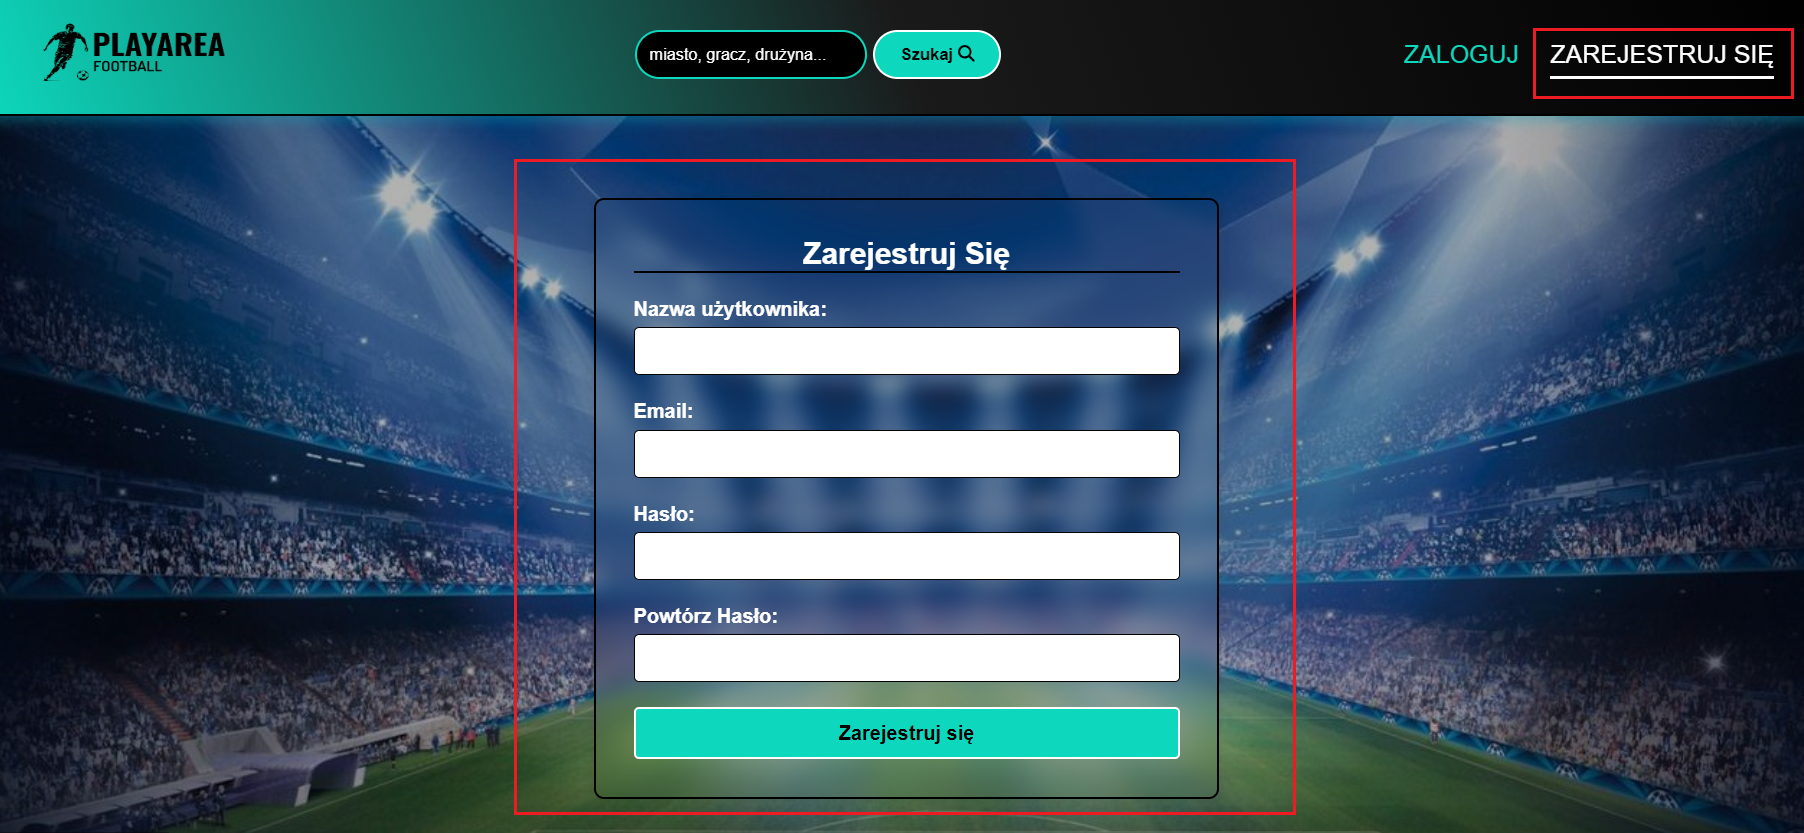
\includegraphics[width=0.9\textwidth]{register.png}
    \caption{Ekran rejestracji - PlayArea}
    \label{fig: ekran_rejestracji}
\end{figure}

\noindent
\noindent Rysunek \ref{fig: ekran_rejestracji} prezentuje ekran, na którym użytkownik może założyć swoje konto. Zawiera pola do wpisania danych, takich jak nazwa użytkownika, e-mail oraz hasło, a także przycisk do zatwierdzenia procesu rejestracji.
\begin{itemize}
    \item \textbf{A. Przycisk "Zrejestruj się"} - po kliknięciu przycisku przenosi użytkownika na ekran rejestracji.
    \item \textbf{B. Pole "Nazwa użytkownika"} - użytkownik wprowadza swoją nazwę użytkownika, w przyszłości ta nazwa będzie także służyć do logowania oraz będzie wyświetlana na profilu użytkownika.
    \item \textbf{C. Pole "Email"} - użytkownik wpisuje swój adres e-mail, który będzie używany do logowania i komunikacji z systemem, e-mail musi byc poprawny aby móc potem potwierdzić rejstrację i dokonać weryfikacji.
    \item \textbf{D. Pole "Hasło"} - użytkownik tworzy hasło dostępu do aplikacji.
    \item \textbf{E. Pole "Powtórz hasło"} - użytkownik ponownie wprowadza hasło w celu weryfikacji, oba hasła muszą się zgadzać.
    \item \textbf{F. Przycisk "Zarejestruj się"} - użytkownik zatwierdza proces rejestracji po wypełnieniu formularza.
\end{itemize}

\section{Logowanie}

\noindent
Ekran logowania cechuje się przejrzystością i intuicyjnością. Wszystkie elementy są wyraźnie rozmieszczone, co ułatwia użytkownikowi szybkie i bezproblemowe wprowadzenie danych. Kolorystyka oraz przyciski nawiązują do ogólnej estetyki aplikacji, zapewniając spójność wizualną.\newline
\begin{figure}[H]
    \centering
    \includegraphics[width=0.9\textwidth]{login.png}
    \caption{Ekran logowania - PlayArea}
    \label{fig: ekran_logowania}
\end{figure}

\noindent Rysunek \ref{fig: ekran_logowania} przedstawia panel logowania, który umożliwia użytkownikom dostęp do swojego konta poprzez wprowadzenie adresu e-mail, nazwy użytkownika oraz hasła. Po prawidłowym uzupełnieniu danych można zalogować się do systemu.
\begin{itemize}
    \item \textbf{A. Pole "Zaloguj"} - po kliknięciu przycisku przenosi użytkownika na ekran logowania.
    \item \textbf{B. Pole "Email"} - służy do wprowadzenia adresu e-mail podanego przy rejestracji w systemie.
    \item \textbf{C. Pole "Nazwa użytkownika"} - służy do wprowadzenia nazwy ustawionej przy rejestracji.    
    \item \textbf{D. Pole "Hasło"} - służy do wprowadzenia hasła, które użytkownik ustawiłprzy rejestracji.
    \item \textbf{E. Przycisk "Zaloguj się"} - po kliknięciu tego przycisku system weryfikuje podane dane logowania i jeśli dane są zgodne loguje nas do systemu.
\end{itemize}

\section{Nawigacja}
\noindent
Pasek nawigacji w aplikacji PlayArea pełni rolę głównego menu, umożliwiając szybki dostęp do różnych sekcji aplikacji. Wyraźne przyciski oraz funkcjonalne rozwijane menu pozwalają użytkownikom zarządzać swoimi drużynami, profilami oraz innymi funkcjami.\newline

\begin{figure}[H]
    \centering
    \includegraphics[width=0.9\linewidth]{navigate.png}
    \caption{Pasek nawigacji - PlayArea}
    \label{fig:navigate}
\end{figure}
\noindent Rysunek \ref{fig:navigate} ilustruje pasek nawigacji, w którym znajdują się przyciski związane z miastem, drużyną oraz profilem użytkownika. Rozwijane menu oferuje dodatkowe opcje, takie jak ustawienia konta, powiadomienia czy możliwość wylogowania.
\newline
\begin{itemize}
    \item \textbf{A. Przycisk "Miasto"} - Wyświetla informacje i opcje związane z aktualnie wybranym miastem oraz ligą istniejącą w tym mieście.
    \item \textbf{B. Przycisk "Drużyna"} - Przenosi użytkownika do sekcji drużyny. W tej sekcji znajdują się główne informacje o drużynie użytkownika.
    \item \textbf{C. Profil użytkownika} - Wyświetla nazwę użytkownika oraz zdjęcie. Po rozwinięciu menu użytkownik ma dostęp do dodatkowych funkcji, takich jak:
        \begin{enumerate}[label=\Roman*., left=0.1cm]
            \item \textbf{Profil gracza} - Przekierowuje do szczegółowego widoku profilu użytkownika.
            \item \textbf{Wyzwij mecz} - Umożliwia wyzwanie innej drużyny na mecz, tą opcję ma dostępną tylko kapitan drużyny.
            \item \textbf{Powiadomienia} - Wyświetla powiadomienia o zaproszeniach do drużyny, jeśli użytkownik jest kapitanem to prośby o przyjęcie do drużyny i zaproszenie do podjęcia meczu z innymi drużynami.
            \item \textbf{Ustawienia} - Pozwala na dostosowanie ustawień konta użytkownika.
            \item \textbf{Wyloguj} - Opcja wylogowania z aplikacji.
        \end{enumerate}
\end{itemize}
\newpage
\section{Strona główna}
\noindent
Strona główna aplikacji została zaprojektowana w sposób przystępny i intuicyjny. Dzięki czytelnym przyciskom użytkownicy mogą szybko przejść do najważniejszych funkcji, takich jak zakładanie drużyny, dołączanie do istniejących zespołów czy przeglądanie rankingów.\newline
\begin{figure}[H]
    \centering
    \includegraphics[width=0.9\linewidth]{home1.png}
    \includegraphics[width=0.9\linewidth]{home2.png}
    \caption{Ekran strony Głównej - PlayArea}
    \label{fig:home}
\end{figure}
\noindent
\newline

\noindent
\noindent Rysunek \ref{fig:home} prezentuje ekran główny, na którym użytkownik ma dostęp do przycisków umożliwiających zakładanie lub dołączanie do drużyn, a także przeglądanie rankingów najlepszych graczy i zespołów w Polsce.
\begin{itemize}
    \item \textbf{A. Przycisk "Załóż drużynę"} - Umożliwia użytkownikowi założenie nowej drużyny w systemie.
    \item \textbf{B. Przycisk "Dołącz do drużyny"} - Pozwala użytkownikowi na dołączenie do istniejącej drużyny po akceptacji przez kapitana.
    \item \textbf{Sekcja "Dlaczego warto grać na PlayArea?"} - Zawiera informacje o głównych funkcjach i zaletach aplikacji, takich jak:
    \begin{itemize}[label=$\cdot$]
        \item \textbf{Rozgrywki 6vs6} - Promuje gry na orlikach i lokalne rywalizacje.
        \item \textbf{Statystyki na żywo} - Śledzenie wyników i statystyk graczy w czasie rzeczywistym.
        \item \textbf{Tabele i rankingi} - Przeglądanie wyników ligowych i statystyk drużyn.
    \end{itemize}
    \item \textbf{C. Tabela Top 10 drużyn w Polsce} - Dzięki tej tabeli możemy śledzić najlepsze drużyny z całej Polski. Ranking bierze pod uwagę ilość meczy, a w drugiej kolejności jeśli ilość meczy jest taka sama pod uwagę jest brany bilans bramek.
    \item \textbf{D. Tabela Top 20 Graczy} - Dzięki tej tabeli możemy śledzić najlepszych graczy z całej Polski. W pierwszej kolejności pod uwagę sąbrane gole, następnie asysty i na końcu liczba MVP.
\end{itemize}

\section{Funkcja szukania}
\noindent
Funkcja wyszukiwania w aplikacji PlayArea została zaprojektowana z myślą o szybkim dostępie do informacji. Użytkownicy mogą z łatwością wyszukiwać miasta, drużyny i graczy z każdego miejsca na stronie, korzystając z dynamicznego mechanizmu filtrowania wyników.\newline
\begin{figure}[H]
    \centering
    
\includegraphics[width=0.9\linewidth]{search.png}
    \caption{Ekran wyszukiwania - PlayArea}
    \label{fig:search}
\end{figure}
\noindent
\newline

\noindent Rysunek \ref{fig:search} przedstawia mechanizm wyszukiwania, który umożliwia użytkownikom wpisanie fragmentu tekstu w celu odnalezienia drużyn, graczy lub miast w systemie. Wyniki wyszukiwania wyświetlają się dynamicznie na ekranie.
\begin{itemize}
    \item \textbf{A. Pole do wpisania} - Umożliwia użytkownikowi wprowadzenie tekstu aby wyszukać daną rzecz. Użytkownik ma możliwość wyszukiwania graczy, miast oraz drużyn, nie musi on także wpisywać całych wyrazów wystarczy ze wpisze część, która jest zawarta w danym wyrazie i zostanie on znaleziony.
    \item \textbf{B. Przycisk "Szukaj"} - po kliknięciu w przycisk, system wyszukuje dany wyraz u wyswietla efekt na ekranie.
    \item \textbf{C. Rezultat wyszukiwań} - służy do wyświetlania rezultatów wyszukiwania,
    może wyświetlać użytkowników, miasta oraz drużyny.
\end{itemize}
\section{Miasto}

\subsection{Widok szczegółowy sekcji Miasto}
Strona "Miasto" przedstawia szczegółowe informacje o wybranej lokalizacji oraz powiązanej lidze. Użytkownicy mogą tutaj przeglądać szczegóły dotyczące miasta, ranking drużyn oraz harmonogram meczów.

\begin{figure}[H]
    \centering
    
\includegraphics[width=0.9\linewidth]{city.png}
    \caption{Widok szczegółowy sekcji Miasto - PlayArea}
    \label{fig:city_details}
\end{figure}

\noindent
Rysunek \ref{fig:city_details} przedstawia ekran wybranego miasta. Użytkownik ma dostęp do szczegółów lokalizacji, takich jak nazwa miasta, województwo, oraz informacje o lidze. Na ekranie wyróżniono następujące elementy:
\begin{itemize}
    \item \textbf{A. Informacje o mieście} - Wyświetla nazwę miasta, województwo oraz szczegóły ligi (np. poziom, numer ligi).
    \item \textbf{B. Przycisk "Tabela"} - Umożliwia przejście do widoku tabeli rankingu sezonu.
    \item \textbf{C. Tabela "Rankingi Sezonu"} - Prezentuje ranking drużyn w wybranej lidze. Dane obejmują miejsce drużyny, liczbę zwycięstw, remisów, porażek, zdobyte i stracone bramki, bilans bramkowy oraz punkty.
\end{itemize}

\subsection{Harmonogram meczów}
Widok harmonogramu meczów umożliwia użytkownikowi śledzenie szczegółów dotyczących przyszłych oraz przeszłych spotkań w ramach ligi.

\begin{figure}[H]
    \centering
    \includegraphics[width=0.9\linewidth]{city2.png}
    \caption{Harmonogram meczów w sekcji Miasto - PlayArea}
    \label{fig:city_matches}
\end{figure}

\noindent
Rysunek \ref{fig:city_matches} przedstawia harmonogram meczów w wybranym mieście. Widok ten podzielono na sekcje, które pokazują szczegółowe informacje o statusie meczów:
\begin{itemize}
    \item \textbf{A. Przycisk "Mecze"} - Umożliwia przełączenie widoku z tabeli rankingu na harmonogram meczów.
    \item \textbf{B. Mecze oczekujące} - Lista meczów oczekujących na zaakceptowanie wyzwania przez kapitanów. Mecze po zaakceptowaniu trafiają do tabeli "Najbliższe mecze", a po odrzuceniu do tabeli "Nieodbyte mecze".
    \item \textbf{C. Najbliższe mecze} - Harmonogram najbliższych spotkań w ramach ligi.
    \item \textbf{D. Ostatnie mecze} - Wyniki ostatnio rozegranych meczów. Wyświetlają się gospodarze, goście oraz końcowy wynik.
    \item \textbf{E. Nieodbyte mecze} - Informacja o meczach, które zostały zaplanowane, ale się nie odbyły, ponieważ któraś z drużyn niezaakceptowała wyzwania.
    \item \textbf{F. Pzycisk strzałki} - Po kliknięciu przycisku użytkownik może przejść do szczegółów meczu oraz przeglądać statystyki zawodników z tego meczu.
\end{itemize}
\section{Drużyna}

\subsection{Widok szczegółowy drużyny}
Widok szczegółowy drużyny przedstawia informacje o wybranej drużynie, takie jak jej nazwa, liczba graczy, statystyki meczów oraz możliwość zarządzania drużyną. Użytkownik, który jest członkiem drużyny, ma dostęp do tych informacji oraz dedykowanych funkcji.

\begin{figure}[H]
    \centering
    
\includegraphics[width=0.9\linewidth]{team.png}
    \caption{Widok szczegółowy drużyny - PlayArea}
    \label{fig:team_details}
\end{figure}

\noindent
Rysunek \ref{fig:team_details} przedstawia widok szczegółowy drużyny w aplikacji PlayArea. Użytkownik ma możliwość przeglądania kluczowych informacji oraz zarządzania drużyną, jeśli posiada odpowiednie uprawnienia. Na ekranie wyróżniono następujące elementy:
\begin{itemize}
    \item \textbf{A. Informacje o drużynie} - Wyświetlają nazwę drużyny, liczbę graczy, liczbę rozegranych meczów, miasto, ligę oraz kapitana drużyny.
    \item \textbf{B. Przycisk "Opuść drużynę"} - Pozwala użytkownikowi na opuszczenie drużyny. Opcja dostępna dla każdego członka drużyny.
    \item \textbf{C. Przycisk "Edytuj drużynę"} - Umożliwia kapitanowi edytowanie szczegółów drużyny, takich jak nazwa, logo czy skład.
    \item \textbf{D. Przycisk "Skład"} - Przenosi użytkownika do widoku składu drużyny, gdzie może przeglądać listę członków oraz ich statystyki.
\end{itemize}

\subsection{Harmonogram meczów drużyny}
Widok harmonogramu meczów umożliwia użytkownikowi śledzenie rozegranych spotkań swojej drużyny.

\begin{figure}[H]
    \centering
d    \includegraphics[width=0.9\linewidth]{team2.png}
    \caption{Harmonogram meczów drużyny - PlayArea}
    \label{fig:team_matches}
\end{figure}

\noindent
Rysunek \ref{fig:team_matches} przedstawia harmonogram meczów drużyny. Na ekranie znajdują się szczegóły dotyczące przeszłych spotkań:
\begin{itemize}
    \item \textbf{A. Przycisk "Mecze"} - Przełącza widok na harmonogram meczów drużyny.
    \item \textbf{B. Lista meczów} - Zawiera szczegóły dotyczące daty, wyniku oraz przeciwników. Każdy mecz wyświetla gospodarzy i gości, a także końcowy wynik.
\end{itemize}

\subsection{Sprawdzenie szczegółów meczu.}
Po kliknięciu w ikonkę strzałki system wyświetla szczegóły meczu.

\begin{figure}[H]
    \centering
    \includegraphics[width=0.9\linewidth]{check_match.png}
    \caption{Harmonogram meczów drużyny - PlayArea}
    \label{fig:check_match}
\end{figure}

\noindent
Rysunek \ref{fig:check_match} przedstawia szczegóły odbytego meczu takie jak, datę spotkania, wynik meczu, drużynę gospodarzy oraz gości, a także graczy poszczególnych drużyn i ich statystyki dotyczące danego meczu.

\section{Profil użytkownika}

Widok szczegółowy profilu użytkownika prezentuje kluczowe informacje związane z jego aktywnością oraz aktualnym stanem w aplikacji. Zawiera szczegóły dotyczące drużyny, wagi, wzrostu, pozycji na boisku oraz numeru zawodnika.

\begin{figure}[H]
    \centering
    \includegraphics[width=0.9\linewidth]{my_profile.png}
    \caption{Widok profilu użytkownika - PlayArea}
    \label{fig:profile_view}
\end{figure}

\noindent
Rysunek \ref{fig:profile_view} przedstawia widok profilu użytkownika w aplikacji PlayArea. Interfejs umożliwia użytkownikowi przegląd jego danych osobistych, aktywności i statystyk. Wybrane elementy widoku to:
\begin{itemize}
    \item \textbf{A. Szczegóły użytkownika} - Prezentuje kluczowe dane użytkownika, takie jak:
    \begin{itemize}[label=$\cdot$]
        \item \textbf{Drużyna} - Nazwa drużyny, do której użytkownik aktualnie należy.
        \item \textbf{Miasto} - Miasto związane z drużyną.
        \item \textbf{Pozycja} - Pozycja zawodnika w drużynie (np. napastnik).
        \item \textbf{Numer} - Numer zawodnika na boisku.
        \item \textbf{Waga i wzrost} - Waga oraz wzrost użytkownika, co może być przydatne dla kapitanów drużyn.
    \end{itemize}
    \item \textbf{B. Statystyki bieżące} - Tabela zawierająca informacje o aktualnych osiągnięciach użytkownika w obecnej drużynie:
    \begin{itemize}[label=$\cdot$]
        \item \textbf{Liga} - Liga, w której uczestniczy drużyna.
        \item \textbf{Gole, asysty i MVP} - Liczba zdobytych goli, wykonanych asyst oraz tytułów MVP (Najbardziej Wartościowy Gracz).
    \end{itemize}
    \item \textbf{C. Statystyki poprzednich drużyn} - Tabela zawierająca dane statystyczne dotyczące drużyn, w których użytkownik grał w przeszłości:
    \begin{itemize}[label=$\cdot$]
        \item \textbf{Drużyna} - Nazwa drużyny, do której użytkownik należał.
        \item \textbf{Liga} - Liga, w której ta drużyna uczestniczyła.
        \item \textbf{Gole, asysty i MVP} - Dane dotyczące liczby goli, asyst oraz zdobytych tytułów MVP w poprzednich drużynach.
    \end{itemize}
\end{itemize}
\section{Wyzwanie meczu}

Widok ekranu umożliwia kapitanowi drużyny rzucenie wyzwania innemu zespołowi na mecz. Interfejs został zaprojektowany w sposób przejrzysty, pozwalający na intuicyjne wypełnienie kluczowych informacji, takich jak wybór drużyny przeciwnika oraz data meczu.

\begin{figure}[H]
    \centering
    \includegraphics[width=0.9\linewidth]{get_challenge.png}
    \caption{Rzucanie wyzwania na mecz - PlayArea}
    \label{fig:challenge_match}
\end{figure}

\noindent
Rysunek \ref{fig:challenge_match} przedstawia ekran umożliwiający rzucenie wyzwania. Interfejs zawiera następujące elementy:
\begin{itemize}
    \item \textbf{A. Informacje o mieście} - Wyświetla szczegóły dotyczące lokalizacji, w której znajduje się liga:
    \begin{itemize}[label=$\cdot$]
        \item \textbf{Miasto} - Nazwa miasta, w którym funkcjonuje liga.
        \item \textbf{Województwo} - Województwo, do którego należy miasto.
        \item \textbf{Liga i poziom} - Informacje o poziomie oraz lidze, w której uczestniczy drużyna.
    \end{itemize}
    \item \textbf{B. Pole wyboru drużyny przeciwnika} - Rozwijane menu pozwalające na wybór zespołu, który użytkownik chce wyzwać na mecz. Dostępne są tylko drużyny z ligi, w której gra drużyna kapitana.
    \item \textbf{C. Pole daty meczu} - Formularz umożliwiający wprowadzenie daty meczu w formacie \texttt{YYYY-MM-DD}. Wprowadzenie daty jest wspomagane przez wbudowany kalendarz.
    \item \textbf{D. Przycisk "Challenge Team"} - Przycisk wysyłający wyzwanie po wypełnieniu wymaganych pól. Po kliknięciu system zapisuje wyzwanie i przesyła powiadomienie do kapitana wybranego zespołu.
\end{itemize}

\section{Powiadomienia}

Widok powiadomień umożliwia użytkownikom przeglądanie, akceptowanie oraz odrzucanie różnych akcji związanych z aplikacją, takich jak prośby o dołączenie do drużyny, zaproszenia do meczu czy inne ważne komunikaty systemowe. Przejrzysty interfejs pozwala szybko podjąć odpowiednie działania.

\begin{figure}[H]
    \centering
    \includegraphics[width=0.9\linewidth]{notification.png}
    \caption{Powiadomienia - PlayArea}
    \label{fig:notifications}
\end{figure}

\noindent
Rysunek \ref{fig:notifications} przedstawia ekran powiadomień w aplikacji PlayArea. Interfejs zawiera następujące elementy:
\begin{itemize}
    \item \textbf{A. Prośba o przyjęcie do drużyny} - Wyświetla szczegóły dotyczące użytkownika, który wysłał prośbę o dołączenie do drużyny:
    \begin{itemize}[label=$\cdot$]
        \item \textbf{Od:} Użytkownik wysyłający prośbę.
        \item \textbf{Do:} Kapitan lub administrator, który ma możliwość zatwierdzenia lub odrzucenia prośby.
        \item \textbf{Wiadomość:} Opis szczegółów prośby o dołączenie.
    \end{itemize}
    \item \textbf{B. Zaproszenie do meczu} - Informacja o wyzwaniu na mecz. Wyświetlane dane obejmują:
    \begin{itemize}[label=$\cdot$]
        \item \textbf{Od:} Kapitan drużyny przeciwnika.
        \item \textbf{Do:} Kapitan drużyny wyzwanego zespołu.
        \item \textbf{Mecz:} Szczegóły dotyczące drużyn oraz daty meczu.
    \end{itemize}
    \item \textbf{C. Zaproszenie do drużyny} - Wyświetla zaproszenie użytkownika do dołączenia do drużyny.
    \item \textbf{D. Akceptuj} - Przycisk umożliwiający zatwierdzenie powiadomienia, np. przyjęcie zaproszenia lub zgody na mecz.
    \item \textbf{E. Odrzuć} - Przycisk pozwalający na odrzucenie zaproszenia lub wyzwania.
    \item \textbf{F. Usuń powiadomienie} - Przycisk usuwający powiadomienie z listy po przetworzeniu lub odrzuceniu akcji.
\end{itemize}
\section{Edycja profilu}

Widok edycji profilu pozwala użytkownikowi na modyfikację danych osobowych oraz ustawień związanych z kontem. Interfejs jest prosty i intuicyjny, umożliwiając szybkie wprowadzenie i zapisanie zmian.

\begin{figure}[H]
    \centering
    \includegraphics[width=0.9\linewidth]{EDIT_PROFILE.png}
    \caption{Edycja profilu - PlayArea}
    \label{fig:edit_profile}
\end{figure}

\noindent
Rysunek \ref{fig:edit_profile} przedstawia ekran edycji profilu użytkownika w aplikacji PlayArea. Interfejs zawiera następujące elementy:
\begin{itemize}
    \item \textbf{A. Awatar użytkownika} - Pole wyświetlające aktualny obraz profilowy użytkownika. Użytkownik może wybrać nowy obraz, który zostanie zapisany jako awatar.
    \item \textbf{B. Przycisk "Zapisz"} - Umożliwia zapisanie zmian w wybranym awatarze użytkownika.
    \item \textbf{C. Przycisk "Usuń trwale konto!"} - Opcja usunięcia konta użytkownika. Po jej wybraniu system wyświetla dodatkowe potwierdzenie przed wykonaniem tej nieodwracalnej operacji.
    \item \textbf{D. Formularz edycji danych} - Zawiera pola do modyfikacji informacji o użytkowniku, takich jak:
    \begin{itemize}[label=$\cdot$]
        \item \textbf{Imię i Nazwisko} - Podstawowe dane użytkownika.
        \item \textbf{Numer} - Numer przypisany użytkownikowi w drużynie.
        \item \textbf{Pozycja} - Rola użytkownika w drużynie (np. napastnik, bramkarz).
        \item \textbf{Waga (kg) i Wzrost (cm)} - Dodatkowe dane o użytkowniku.
        \item \textbf{Miasto} - Lokalizacja użytkownika.
    \end{itemize}
    \item \textbf{E. Przycisk "Zapisz zmiany"} - Zatwierdza i zapisuje wprowadzone zmiany w danych użytkownika.
    \item \textbf{F. Przycisk "Powrót"} - Pozwala użytkownikowi wrócić do poprzedniego widoku bez zapisywania zmian.
\end{itemize}
\section{Potwierdzenie wyniku meczu}

Ekran potwierdzenia wyniku meczu umożliwia wprowadzenie oraz weryfikację wyników rozgrywki przez kapitana drużyny. Użytkownik wprowadza szczegółowe dane, takie jak liczba zdobytych goli, asyst oraz wybiera najbardziej wartościowego gracza (MVP). System weryfikuje poprawność danych przed ich zatwierdzeniem.

\begin{figure}[H]
    \centering
    \includegraphics[width=0.9\linewidth]{confrim_match.png}
    \caption{Potwierdzenie wyniku meczu - PlayArea}
    \label{fig:confirm_match}
\end{figure}

\noindent
Rysunek \ref{fig:confirm_match} przedstawia ekran potwierdzenia wyniku meczu w aplikacji PlayArea. Interfejs zawiera następujące elementy:
\begin{itemize}
    \item \textbf{A. Sekcja "Kozaki (Gospodarze)"} - Pole umożliwiające wprowadzenie liczby zdobytych goli przez drużynę gospodarzy oraz przypisanie statystyk do poszczególnych graczy.
    \item \textbf{B. Sekcja "United (Goście)"} - Pole umożliwiające wprowadzenie liczby zdobytych goli przez drużynę gości. Tutaj można również przypisać gole, asysty oraz wybrać MVP dla graczy z tej drużyny.
    \item \textbf{C. Kolumna "Gole"} - Służy do wprowadzenia liczby goli przypisanych poszczególnym graczom. System automatycznie sumuje te wartości.
    \item \textbf{D. Kolumna "Asysty"} - Pole do wprowadzenia liczby asyst przypisanych każdemu graczowi.
    \item \textbf{E. Kolumna "MVP"} - Opcja wyboru najbardziej wartościowego gracza (MVP) z danej drużyny poprzez zaznaczenie odpowiedniego pola.
    \item \textbf{F. Przycisk "Zatwierdź wynik"} - Służy do zapisania wprowadzonych danych. System sprawdza poprawność wprowadzonych informacji przed ich ostatecznym zapisaniem.
    \item \textbf{G. Komunikat o błędzie} - Wyświetla ostrzeżenie w przypadku rozbieżności między liczbą goli przypisaną poszczególnym graczom a wynikiem drużyny.
\end{itemize}
\chapter{Podsumowanie}
Praca miała na celu stworzenie aplikacji PlayArea, która stanowi nowoczesne narzędzie do zarządzania amatorskimi ligami piłkarskimi. Projekt łączy w sobie potrzeby organizatorów, kapitanów drużyn oraz zawodników, oferując intuicyjne rozwiązanie do organizacji meczów, wprowadzania wyników oraz śledzenia statystyk. Dzięki zastosowaniu technologii takich jak React.js, Django, GraphQL i SQLite, udało się stworzyć wydajny, skalowalny i przyjazny użytkownikowi system.

Przeprowadzono analizę konkurencyjnych platform, takich jak Playarena.pl i Podlaska Liga Sportowa, aby zidentyfikować kluczowe funkcjonalności i luki, które mogłyby zostać wypełnione przez PlayArea. Na tej podstawie opracowano unikalne cechy aplikacji, takie jak moduł powiadomień, dynamiczne wyszukiwanie drużyn i zawodników oraz mechanizm potwierdzania wyników meczów. Aplikacja wspiera organizację lokalnych lig, redukując czas i wysiłek potrzebny do zarządzania nimi, a jednocześnie promuje zdrowy styl życia i rozwój społeczności sportowych.

PlayArea to praktyczne narzędzie, które w prosty i przejrzysty sposób integruje organizację rozgrywek amatorskich, czyniąc je bardziej dostępnymi i atrakcyjnymi zarówno dla drużyn, jak i poszczególnych graczy.

\chapter*{Streszczenie}

Celem pracy było zaprojektowanie i stworzenie aplikacji webowej PlayArea, która wspiera zarządzanie ligami amatorskimi, koncentrując się na uproszczeniu procesu organizacji rozgrywek piłkarskich. Aplikacja umożliwia użytkownikom dołączanie do drużyn, tworzenie nowych zespołów, zarządzanie harmonogramami meczów, wprowadzanie wyników oraz śledzenie szczegółowych statystyk zarówno drużynowych, jak i indywidualnych. Dzięki intuicyjnemu interfejsowi użytkownika oraz nowoczesnym technologiom, takim jak React.js, Django i GraphQL, aplikacja oferuje wydajne i skalowalne rozwiązanie dla lokalnych społeczności sportowych.

W pracy przeanalizowano istniejące platformy, takie jak Playarena.pl i Podlaska Liga Sportowa, by zidentyfikować ich zalety i ograniczenia. Na tej podstawie opracowano unikalne funkcje, takie jak dynamiczne wyszukiwanie drużyn i zawodników, moduł powiadomień oraz kompleksowy system potwierdzania wyników meczów. Aplikacja PlayArea wspiera rozwój lokalnych lig, upraszczając proces organizacji rozgrywek i promując aktywność fizyczną w społecznościach.

\chapter*{Abstract}

The goal of this thesis was to design and develop a web application called PlayArea to streamline the management of amateur football leagues. The application simplifies the organization of matches by enabling users to join teams, create new squads, manage match schedules, input results, and track detailed statistics for teams and individual players. Leveraging modern technologies like React.js, Django, and GraphQL, the application provides an efficient and scalable solution for local sports communities.

The study also includes an analysis of existing platforms such as Playarena.pl and Podlaska Liga Sportowa to identify their strengths and weaknesses. Based on this analysis, PlayArea introduces unique features like dynamic search for teams and players, a notification module, and a comprehensive match result confirmation system. This application supports the growth of local leagues by simplifying organizational processes and promoting physical activity within communities.
\listoffigures
\listoftables
\end{document}
